\documentclass[11pt]{article}
\usepackage{physics}
% NOTE: Add in the relevant information to the commands below; or, if you'll be using the same information frequently, add these commands at the top of paolo-pset.tex file. 
\newcommand{\name}{TA: Hossein Mohammadi}
\newcommand{\email}{hossein.mohammadi.00427@gmail.com}
\newcommand{\classnum}{Advanced Quantum Field Theory}
\newcommand{\subject}{Subject: Path Integrals}
\newcommand{\instructors}{Dr. Amin Faraji}
\newcommand{\assignment}{PSet 2}
\newcommand{\semester}{- Fall 1402}
\newcommand{\duedate}{dd/mm/yyyy}
\input{paolo-pset.tex}

% NOTE: To compile a version of this pset without problems, solutions, or reflections, uncomment the relevant line below.

%\excludeversion{problem}
%\excludeversion{solution}
%\excludeversion{reflection}

\begin{document}	
	
	% Use the \psetheader command at the beginning of a pset. 
	\psetheader
	
	\section*{Problem 1: Grassmannian Path Integrals }
	
	\begin{problem}
		In this problem, we will review some essential concepts regarding non-commutative path integrals.
	\end{problem}
	\begin{enumerate}
		\item
		\begin{problem}{\points[9.5 Peskin]{-}}
			\textbf{Basic properties of Grassmann numbers:}
			
			\noindent
			The basic fact about these numbers is that they anti-commute, $\eta\theta = -\theta \eta$. Hence they square to zero, $\theta^2 = 0$.‌ Argue that any function of Grassmann number is a linear function, $f(\eta) = A\eta+B$.
			
			\noindent
			\textbf{Aside:} In light of $\theta^2=0$, can we conclude that terms such as $\bar{\psi} \psi \bar{\psi} \psi$ or $(\bar{\psi}\psi)^2$ vanish in Lagrangian? As an instance, 4-Fermi theory has the former term.
		\end{problem}
		\item
		\begin{problem}{\points[9.5 Peskin]{-}}
		\textbf{Integration of Grassmann valued functions:}
		
		We define $\int d\theta (A+B\theta) = B$. Justify this definition by considering a change of variable $\theta \xrightarrow{} \theta + \eta$.
		\end{problem}
	\item
	\begin{problem}{\points[9.5 Peskin]{-}}
		\textbf{A simple Integration:}
		
		\noindent
		Let's play more with this interesting variables.

		\begin{enumerate}
			\item To warm up, compute $\int d\bar{\theta}d\theta e^{-\bar{\theta}b\theta}$, where $b$ is an ordinary number.[ Just expand this integral and use the $\theta^2= \bar{\theta}^2 =0$ property.]
			\item Compute $\int d\bar{\theta}d\theta\;\bar{\theta}\theta e^{-\bar{\theta}b\theta}$, where $b$ is an ordinary number.[ Notice the importance of ordering of Grassmann variables, unless we will have a minus ambiguity.]
			\item To generalize to multi-variable case, consider the following integral:
			\[
			\int d\bar{\theta}_1 \dots  d\bar{\theta}_n d\theta_1 \dots d\theta_n e^{-\bar{\theta}_i A_{ij} \theta_j}
			\]
			Where $A_{ij}$ is a $n\times n$ matrix. Work out this formula. [Expand the exponential and decide which terms survive. You must end up to $\det(A)$.]
			\item $[\text{Optional}]$ Another way of doing this, as Peskin does, is utilizing defintion of Jacobian of transformation in the Grassmann variables. This is a simple exercise that could be accompllished.

			
		\end{enumerate}
	\end{problem}
\end{enumerate}



\newpage

\section*{Problem 2: Path Integral Manual Dexterity}
\begin{problem}
	In this problem, we use all our knowledge to quantize elementary theories by path integrals. 
	Scalar QED and establishing the equivalence of correlation functions in second-quantized and path integral quantizations, are subjects of this exercise.
\end{problem}	

	\begin{enumerate}
	\item
	\begin{problem}{\points[Peskin Problem 9.1]{-}}
		\textbf{Scalar QED:} 
		
		\noindent
		This problem concerns the scalar QED theory of a complex field $\phi$ interacting with the electromagnectic potential $A^\mu$. The lagrangian is 
		\[
		\mathscr{L} = -\frac14 F_{\mu\nu}^2 + (D_\mu \phi)^{*} (D^\mu\phi) - m^2\phi^{*}\phi
		\]
		Where $D_\mu = \partial_\mu + ieA_\mu$.
		
		\noindent
		Use the functional methods discussed in Section 9.2, show that the following are Feynmann rules of this theory.
		
		\begin{figure}[H]
			\centering
			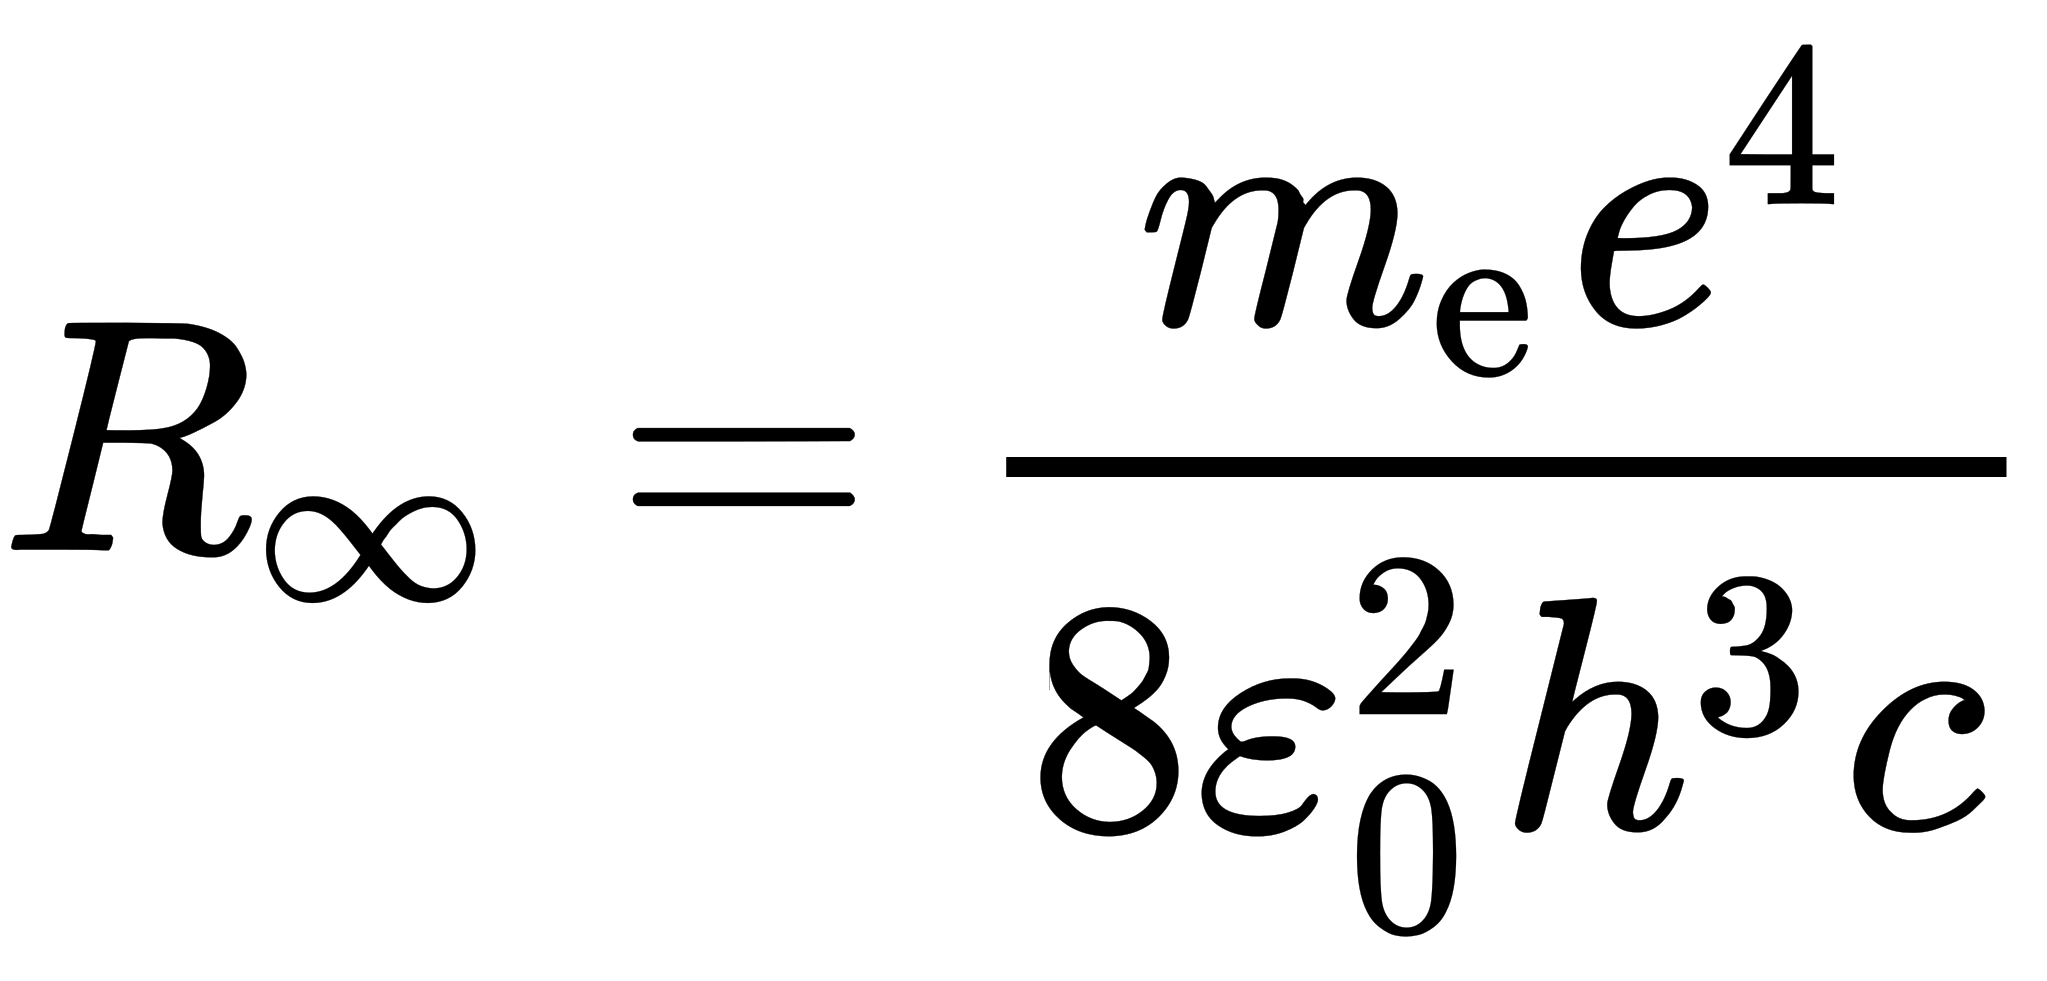
\includegraphics[width=0.5\linewidth]{img/1.png}
			\caption{Scalar QED basic Feynman diagrams.}
		\end{figure}
	\end{problem}
	\item
	\begin{problem}{\points{-}}
		\textbf{Correlation functions in different quantization schemes}
		
		\noindent
		 We want to establish the equivalence between n-point functions in second-quantization and path integal quantization.
		 
		\noindent
		\begin{enumerate}
			\item 
			Using what we've learned in the classroom about generating functionals and sources $J$, prove that second quantized n-point function 
			\[
			\bra{\Omega} T{\phi(x_1) \dots \phi(x_n)} \ket{\Omega} = \frac{
		\bra{0} T\{\phi_0(x_1) \dots \phi_0(x_n) e^{i\int d^4x \mathscr{L}_{int}[\phi]}\}\ket{0}	
		}{
\bra{0} T\{ e^{i\int d^4x \mathscr{L}_{int}[\phi]}\}\ket{0}		
}
			\],
			is equivalent to 
			\[
			(-i)^n \frac{1}{Z[0]} \frac{\partial^n Z}{\partial J(x_1) \dots \partial J(x_n)} \Big|_{J=0}
			\].
			In first relation $\phi_0(x)$ is the Heisenberg picture fields in free-theory and in the second, $Z[J]$ is generating functional of the full theory.
			
			\noindent
			[Despite its formidable appearance, it's a trivial question. Don't be afraid and start by divding full Lagrangian into $\mathscr{L} = \mathscr{L}_{free} + \mathscr{L}_{int}$, then plug it into path integral and use the relation between path-integral and n-point function in "Free Theories".]
			
			\item  Now that you've proved the most general case, let's verify it for $\phi^3$ theory, where $\mathscr{L}_{int} = \frac{g}{3!} \phi^3$. Expand $e^{i\int d^4 \mathscr{L}_{int}}$ in the path integral and conclude that two point function in this interactive theory gives the same result as Feynman rules up to order $g^4$.
		\end{enumerate}
	\end{problem}





\end{enumerate}


\newpage
\section*{Problem 3: Quantum Statistical Mechanics}
\begin{problem}
	We work out the world's most famous problem in the path integral formalism. These problems are 9.2 (a) and (b), Peskin.
\end{problem}	

\begin{enumerate}
	\item
	\begin{problem}{\points[Peskin Problem 9.2 (a)]{-}}
		\textbf{Quantum Statistical Mechanics} 
		
		\noindent
		Solve problem 9.2 (a), which is a review of quantum mechanical path integral, but in Euclidean signature.
	\end{problem}
	\item
	\begin{problem}{\points[Peskin Problem 9.2 (b)]{-}}
		\textbf{Harmonic Oscillator Path Integral}
		
		\noindent
	Now work out the part (b). Use the fourier expansion suggested, plug into path integral. The integration is a bit baffling, but pay close attention to (9.23) to figure out how to do these integrals. You will eventally end up with an infinite product, which turns out to be $\sinh(z)$, as suggested in the question. This gives the correct partition function for quantum mechanical oscillators, one that you've read in advanced statistical mechanics courses.
	\end{problem}
	
	
	
	
	
\end{enumerate}






\noindent
\begin{reflection}
	There are many interesting ideas in path integrals:
	\begin{itemize}
		\item  Schwinger Dyson equations: this equations govern the expectation values of the field operators, and bear a close resemblance to classical counterparts up to contact terms.
		\item Noether current and other symmetries: this is surprising how a simple change of variables in path integral could give us Noether current and Ward-Takahashi identity in QED.
		\item Quantization of QED: this is also a general procedure to quantize spin-1 fields, discussed in your textbook, I hope you cover these parts too.
	\end{itemize}
\end{reflection}

\end{document}